\subsection{EVL+STrace}
\label{sec:EVLPlusSTrace}

The bx tool \emph{EVL+STrace} \cite{IST2018-Samimi} is based on EMF as well as the \emph{Epsilon} framework \cite{epsilon}, which provides tool support for a variety of DSLs for model transformation.
In EVL+STrace, a transformation definition consists of a trace metamodel, EOL operations, and EVL constraints (figure~\ref{fig:evlartefacts}).

The \emph{trace metamodel} defines domain-specific types of links and link ends.
Trace models contain copies of all relevant elements of source and target models, as well as links connecting these elements.
By means of a rich trace model, it is possible to detect any category of changes to the participating models, including creation and deletion of objects and links, as well as modification of attribute values.

The behavior of the synchronizer is defined by \emph{EOL operations}, i.e., operations for queries and updates written in the Epsilon Object Language, and \emph{EVL constraints}, i.e., checks augmented with repair actions written in the Epsilon Validation Language.
Each constraint is directed and checks an inconsistency between the trace model and one of the participating models which is caused by a change to this model.
The corresponding repair action propagates this change to the trace model and the opposite model.

\begin{figure}[tb!]
	\centering
	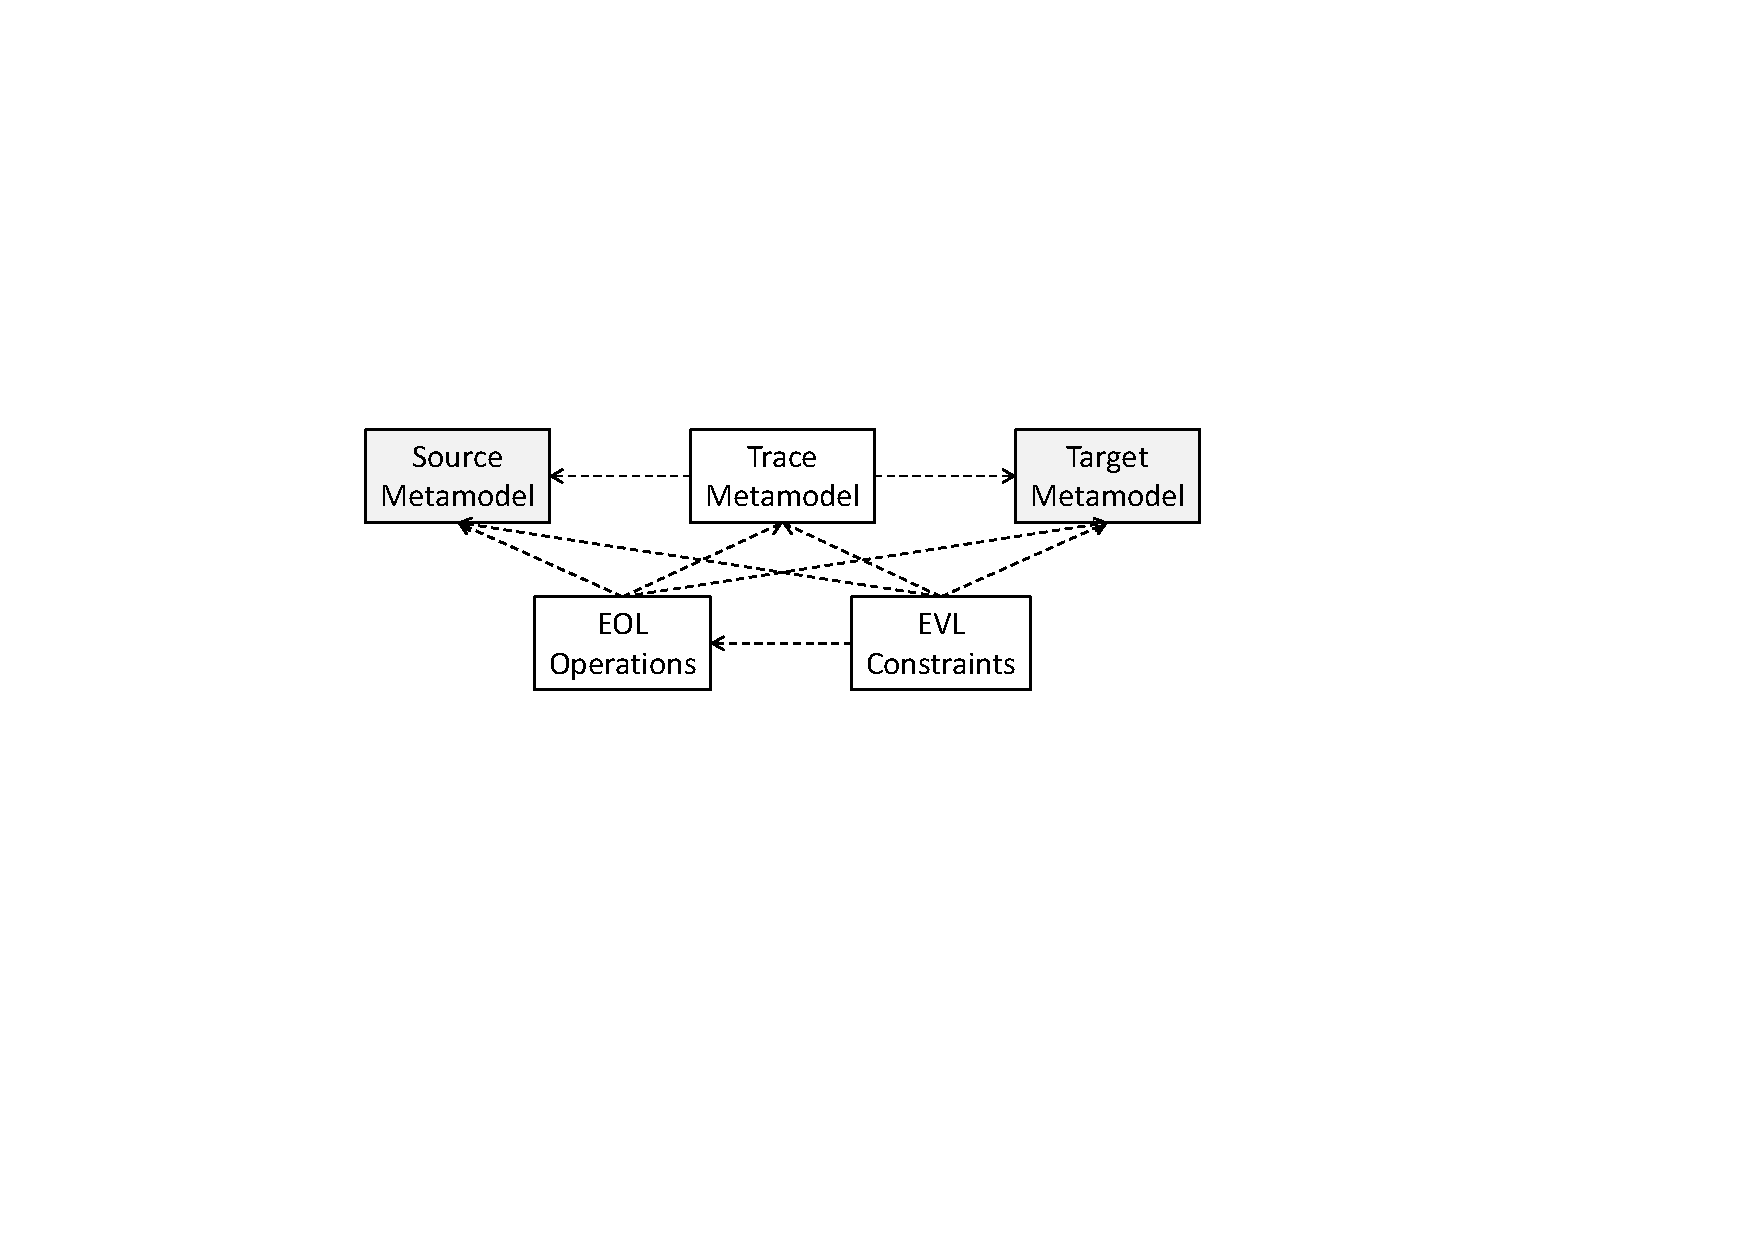
\includegraphics[width=0.8\columnwidth]{diagrams/solutions/EVLPlusSTraceArtefacts}
	\caption{EVLPlusSTrace artefacts and their dependencies}
	\label{fig:evlartefacts}
\end{figure}

\begin{figure*}[tb!]
	\centering
	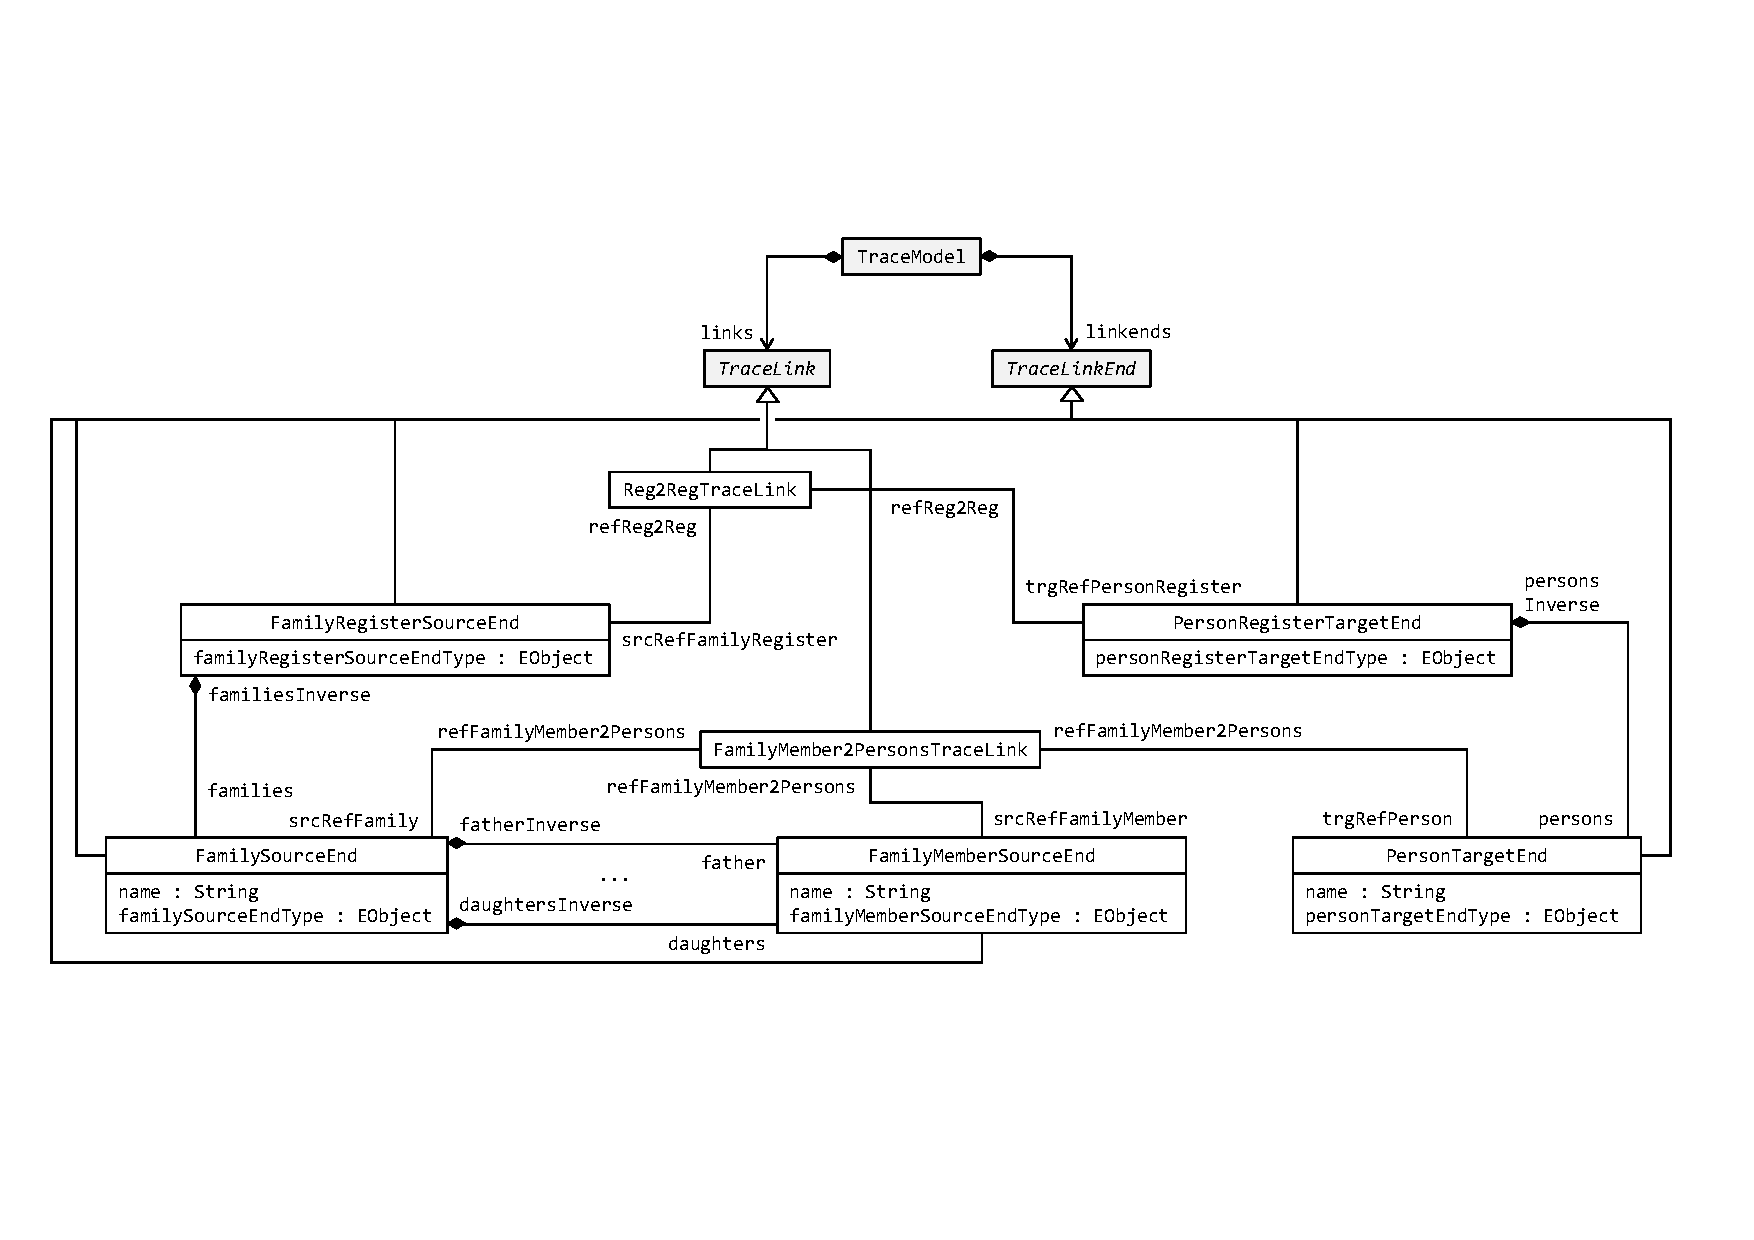
\includegraphics[width=\textwidth]{diagrams/solutions/EVLPlusSTraceMetamodel}
	\caption{Trace metamodel for Families to Persons (without multiplicities)}
	\label{fig:evltracemetamodel}
\end{figure*}

\subsubsection{Classification}
\label{sec:ClassificationEVL}

EVL+STrace is \emph{restoration-based}: the transformation developer specifies how to detect and repair inconsistencies by explicitly programming \emph{fCR} and \emph{bCR}.
With respect to horizontal and vertical inputs, EVL+STrace is classified as \emph{initial-diag-based} and realizes the tool architecture displayed in figure~\ref{fig:initialDiagBased} on the left-hand side. 

As the transformation developer is free to implement both consistency checks and repairs, adherence to any formal property cannot be guaranteed in general. 
For example, an update that changes the trace model but preserves consistency can be responded to by an -- according to hippocraticness unnecessary -- repair action.
Correctness is also not guaranteed: repair actions are specified in a procedural way and may fail to restore consistency or can contradict the checks for consistency.

In EVL+STrace, the \emph{consistency relation} is defined \emph{explicitly} as a set of  \emph{constraints}.
The overall consistency relation is composed of two sets of directed constraints; the transformation developer is responsible for the mutual consistency of forward and backward constraints.
Constraint restoration is also explicitly specified and controlled by programmed repair operations.

EVL+Strace is designed primarily for \emph{concurrent synchronization}, i.e., consolidating  changes applied to both participating models.
Directed synchronization is included as a special case: If only one of the participating models has been modified, constraints may be violated only between this model and the trace model.

Synchronization is performed \emph{on demand} and \emph{interactively}: Each constraint violation is reported to the user, who has to confirm (or reject) the respective repair action.
Automatic synchronization is possible, but requires rewriting of EVL constraints (explained in the following section).

\subsubsection{Benchmark solution with EVL+STrace}
\label{sec:solutionEVL}

The following description is based on the solution in EVL+STrace submitted to TTC 2017 \cite{Samimi-Dehkordi2017}.
Figure~\ref{fig:evltracemetamodel} displays the \emph{trace metamodel} for the Families to Persons benchmark. Specific types of trace links and trace link ends are defined by subclassing built-in abstract superclasses \code{TraceLink} and \code{TraceLinkEnd}, respectively. Each \emph{trace link} references a set of trace link ends, which may be considered proxies of source or target model objects. \emph{Trace link ends} store links to source or target model objects with the help of attributes of type \code{EObject}. In addition, trace link ends may store attribute values and may be connected by links. In this way, the trace model may shadow the relevant parts of the source and target models. In the case of the Families to Persons benchmark, the trace metamodel defines two types of trace links for relating family and person registers as well as for relating family members along with their families with persons.


 
\lstdefinelanguage{evl}{
	morekeywords = {context,constraint,guard,not,self,check,message,fix,title,do,var,if,else,delete},
	morecomment=[l]{//},
	morecomment=[s]{/*}{*/}
}


\begin{lstlisting}[label={lst:evl}, float=b!, language=evl, caption={Example of an EVL constraint}]
context Source!FamilyMember{
  constraint isNewMale{
    guard: self.isMale()
    check: not self.isNew()
    message:self+' is a new inserted element 
      in the source model'
    fix{
      title:'Insert its corresponding elements 
        in the trace and target models'
      do {
        var familyMemberSourceEnd 
          = addFamilyMemberSourceEnd(self);
        var family;
        if(self.isFather()) 
          family = self.fatherInverse;
        else 
          family = self.sonsInverse;
        family.satisfies("isNew");
        var familySourceEnd 
          = family.getTraceLinkEnd(); 
        if(self.isFather()) 
          familyMemberSourceEnd
            .setFatherInverse(familySourceEnd);			
        else 
          familyMemberSourceEnd
            .setSonsInverse(familySourceEnd);			
        var person = insertMale(family,self);
        var personTargetEnd 
          = addPersonTargetEnd(person);
        addFamilyMember2PersonsTraceLink(
          familySourceEnd, 
          familyMemberSourceEnd, 
          personTargetEnd);
        copySrc2Trg();
      }
    }
  }
}
\end{lstlisting}

Listing~\ref{lst:evl} gives an example of an \emph{EVL} constraint along with its repair action. The constraint refers to family members in the families models (line~1).
As indicated by the name of the constraint (line~2), it handles the creation of a new male member.
Its guard (line~3) ensures that it may be applied only to male family members.
The check (line~4) defines that the member must not be new, i.e., there must be a corresponding person in the persons model.
If this check fails, a meaningful message (line~5--6) is created and displayed in the user interface.
The fix (line~7--36) has a title (line~8--9) explaining the repair action to the user, as well as a \code{do} part (starting at line~10) which defines all operations to restore consistency in a procedural way.
Note that these operations refer both to the persons model and the trace model.

The Families-to-Persons benchmark deviates from the primary synchronization scenario targeted by EVL\-+\-STrace in two respects.
First, the benchmark comprises only alternating direct rather than concurrent changes, i.e., only one model is changed, and the opposite model is updated to restore consistency.
Second, the test suite is executed automatically, without any user interaction.
%
As EVL+STrace is designed to support the more general case of concurrent synchronization, it can of course also handle the simplified case of directed synchronization.
For automatic synchronization, the constraint definitions have to be modified by moving the \code{do} part into the \code{check} part, as well as eliminating the \code{message} and the \code{fix} parts.
These mechanical transformations were applied throughout the EVL code to execute the Families-to-Persons benchmark without user interaction.


%%% Local Variables:
%%% mode: latex
%%% TeX-master: "../main"
%%% End:
